%compile with pdflatex on papeeria

\documentclass[a4paper,12pt]{article}
\usepackage{fancyhdr}
\usepackage{fancyheadings}
\usepackage[ngerman,german]{babel}
\usepackage{german}
\usepackage[utf8]{inputenc}
%\usepackage[latin1]{inputenc}
\usepackage[active]{srcltx}
%\usepackage{algorithm}
%\usepackage[noend]{algorithmic}
\usepackage{amsmath}
\usepackage{amssymb}
\usepackage{amsthm}
\usepackage{bbm}
\usepackage{enumerate}
\usepackage{graphicx}
\usepackage{ifthen}
\usepackage{listings}
\usepackage{enumitem}
%\usepackage{struktex}
\usepackage{hyperref}
\usepackage{tikz}
\usepackage{float}
\usepackage{subcaption}
\captionsetup{compatibility=false}
\captionsetup[subfigure]{labelformat=empty}

\usepackage{pgfplots}
\pgfplotsset{compat=1.15}
\usepackage{mathrsfs}
\usetikzlibrary{arrows}

\definecolor{ccqqqq}{rgb}{0.8,0,0}

\pagenumbering{gobble}

%%%%%%%%%%%%%%%%%%%%%%%%%%%%%%%%%%%%%%%%%%%%%%%%%%%%%%
%%%%%%%%%%%%%% EDIT THIS PART %%%%%%%%%%%%%%%%%%%%%%%%
%%%%%%%%%%%%%%%%%%%%%%%%%%%%%%%%%%%%%%%%%%%%%%%%%%%%%%
\newcommand{\Fach}{1. Klausur aus der Mathematik (A)}
\newcommand{\Name}{}
\newcommand{\datum}{}
\newcommand{\Matrikelnummer}{}
\newcommand{\Semester}{Q11/1}
\newcommand{\Uebungsblatt}{} %  <-- UPDATE ME
%%%%%%%%%%%%%%%%%%%%%%%%%%%%%%%%%%%%%%%%%%%%%%%%%%%%%%
%%%%%%%%%%%%%%%%%%%%%%%%%%%%%%%%%%%%%%%%%%%%%%%%%%%%%%

\setlength{\parindent}{0em}
\topmargin -1.0cm
\oddsidemargin 0cm
\evensidemargin 0cm
\setlength{\textheight}{9.2in}
\setlength{\textwidth}{6.0in}

%%%%%%%%%%%%%%%
%% Aufgaben-COMMAND
\newcommand{\Aufgabe}[1]{
  {
  \vspace*{0.5cm}
  \textsf{\textbf{Aufgabe #1}}
  \vspace*{0.2cm}
  
  }
}
%%%%%%%%%%%%%%
\hypersetup{
    pdftitle={\Fach{}: Übungsblatt \Uebungsblatt{}},
    pdfauthor={\Name},
    pdfborder={0 0 0}
}

\lstset{ %
language=java,
basicstyle=\footnotesize\tt,
showtabs=false,
tabsize=2,
captionpos=b,
breaklines=true,
extendedchars=true,
showstringspaces=false,
flexiblecolumns=true,
}

\title{Übungsblatt \Uebungsblatt{}}
\author{\Name{}}

\begin{document}
\thispagestyle{fancy}
%\lhead{\sf \large \Fach{} \\ %\small \Name{} - \Matrikelnummer{}
\lhead{\sf \large \Fach{} %\small \Name{} - \Matrikelnummer{}
}
\rhead{\sf \Semester{}   \datum{}}
%\rhead{\sf \Semester{} }
\vspace*{0.2cm}
%\begin{center}
%%\LARGE \sf \textbf{Übungsblatt \Uebungsblatt{}}
%\end{center}
%\vspace*{0.2cm}

%%%%%%%%%%%%%%%%%%%%%%%%%%%%%%%%%%%%%%%%%%%%%%%%%%%%%%
%% Insert your solutions here %%%%%%%%%%%%%%%%%%%%%%%%
%%%%%%%%%%%%%%%%%%%%%%%%%%%%%%%%%%%%%%%%%%%%%%%%%%%%%%

  Name: \underline{\hspace{7cm}}
  \hfill
  Datum: \underline{\hspace{4cm}}

%\vspace{0,5cm}Die Rechenwege müssen nachvollziehbar sein!
%
%\vspace{0,5cm} {TEIL A} - ohne Hilfsmittel - Bearbeitungszeit 30 Minuten
%\vspace {0,2cm}
% 
%GEOMETRIE

\Aufgabe{1} 


%\begin{tabular}{|p{0.18cm}|m{0.18cm}|b{0.18cm}|l|}
%\hline
%a\newline a & b\newline b & c\newline c\newline c& d \\
%\hline
%\end{tabular}


\begin{enumerate}[label={\alph*)}]
\item Geben Sie den Term einer Funktion $f$ an, deren Steigung immer konstant ist.
\item Beschreiben Sie in einem Satz die Bedeutung der lokalen Änderungsrate in dem untensthenden Beispiel. \\

  \begin{tabular}{|c|c|}
    \hline
    Größe F (Einheit von F) & Lokale Änderungsrate der Größe F \\[2.5ex] \hline 
    Länge einer Pflanze (cm) & ? \\[2.5ex] \hline
  \end{tabular}
  
%\begin{center}
%\end{center}
\item Bestimmen Sie den Steigungswinkel der Tangente $t$ mit
  $ y_t = -\frac{1}{3}x + 7$
,den diese mit der $x$-Achse einschließt. Runden Sie auf ganze Grad.
\item Eine Tangente berührt den Graphen der Funktion $f: x \rightarrow 0,5x^2 - 11$
an der Stelle $x_0 = 4$. Bestimmen Sie die Gleichung der Normalen, welche auf dieser Tangente senkrecht steht.
\end{enumerate}
\begin{flushright}8 BE \end{flushright}

\Aufgabe{2:} 
Gegeben ist die Funktion $f: x \rightarrow \frac{x^2}{9-3x}$
\begin{enumerate}[label={\alph*)}]
  \item Geben Sie die maximale Definitionsmenge $D_f$ und die Nullstellen von $f$ an.\\
Die Funktion $f$ lässt sich auch in der Form
    $f(x) = - \frac{1}{3}x - 1 + \frac{3}{3-x}$ 
darstellen (kein Nachweis erforderlich).


\item Untersuchen Sie das Verhalten an den Rändern der Definitionsmenge und geben Sie die Gleichungen aller Asymptoten des Graphen an!
\item Ermitteln Sie das Monotonieverhalten und die Lage und Art der Extrema der Funktion.\\
 \lbrack Zur Kontrolle: $f'(x) = (-3x^2+18x) / (9-3x)^2$\rbrack

\marginpar{
  \begin{center}
Platzbedarf:
7\\
8 11\\
8\\
  \end{center}
}
\item Skizzieren Sie den Graphen von $f$ unter Verwendung der bisherigen Ergebnisse.

\end{enumerate}
\begin{flushright}17 BE \end{flushright}

  \newpage
\Aufgabe{3:}

Bei einer bestimmten chemischen Reaktion wird die zeitliche Änderung der Konzentration $c$ eines Stoffes mit einer Anfangskonzentration von $c_0=0,125 \frac{mol}{l}$ beschrieben durch das Gesetz $c(t) = \frac{1}{7,7t+\frac{1}{0,145}}$\\
$t$ bezeichnet dabei die seit Beginn der Reaktion vergangene Zeit in Minuten.
\begin{center}
    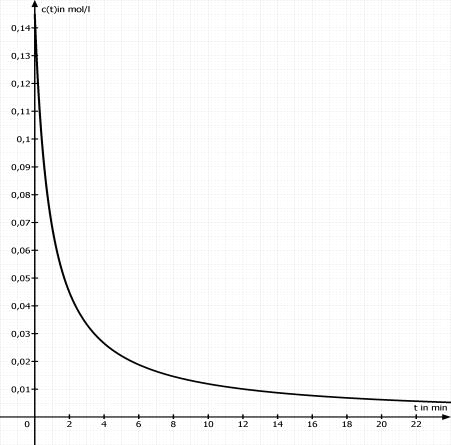
\includegraphics[width=0.6\linewidth]{Q11_210111_3corrected.jpg}
\end{center}

%\begin{figure}[h!]
%  \begin{center}
%    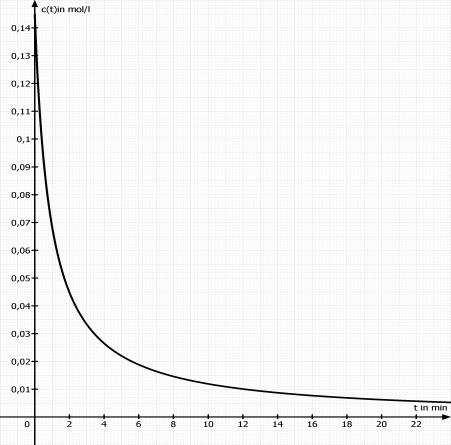
\includegraphics[width=0.7 \linewidth]{Q11_210111_3.jpg}
%  \end{center}
%\end{figure}


\begin{enumerate}[label={\alph*)}]
\item Berechnen Sie allgemein die momentane Änderungsrate der Konzentration.
\item Bestimmen Sie nun die momentane Änderungsrate der Konzentration zu Beginn und nach zehn Minuten der Reaktion. Achten Sie auf die korrekte Einheit!\\
  \lbrack Verwenden Sie, falls sie a) nicht lösen konnten:
    $c'(t) = -\frac{7,7}{59,3t^2+106,2t+47,6}$\rbrack

\item Geben Sie die mittlere Änderungsrate in den ersten zehn Minuten an und begründen Sie, warum sich dieser Wert von $c’(10)$ unterscheidet.

\end{enumerate}

\begin{flushright}9 BE \end{flushright}

\Aufgabe{4:}

\begin{minipage}{0.5\linewidth}
Gegeben ist der Graph einer Funktion $f$:\\

Welcher der folgenden Graphen kann der Graph der Ableitung von $f$ sein?\\

Begründen Sie Ihre Entscheidung anhand von \underline{zwei} verschiedenen Eigenschaften!\\

Geben Sie \underline{jeweils einen} Grund an, warum die übrigen Graphen nicht die Ableitung von $f$ darstellen können!

\end{minipage}\hfil
\begin{minipage}{0.5\linewidth}
    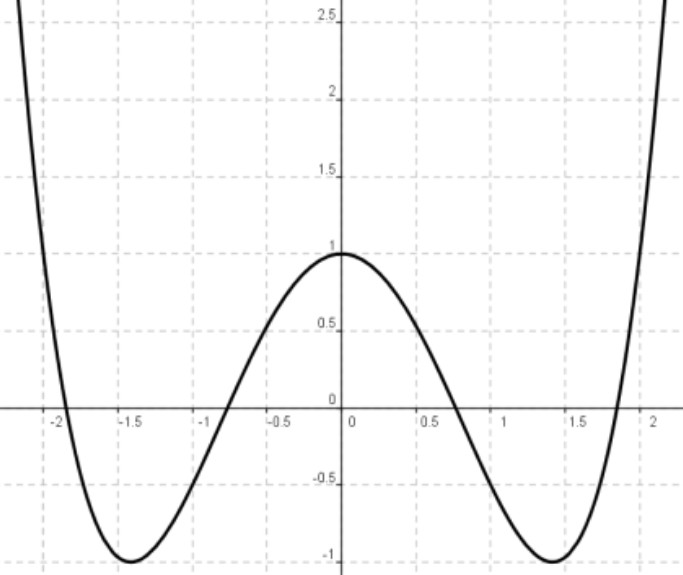
\includegraphics[width=0.8\linewidth]{Q11_210111_4.jpg}
\end{minipage}


%\begin{figure}[h!]
%  \begin{center}
%    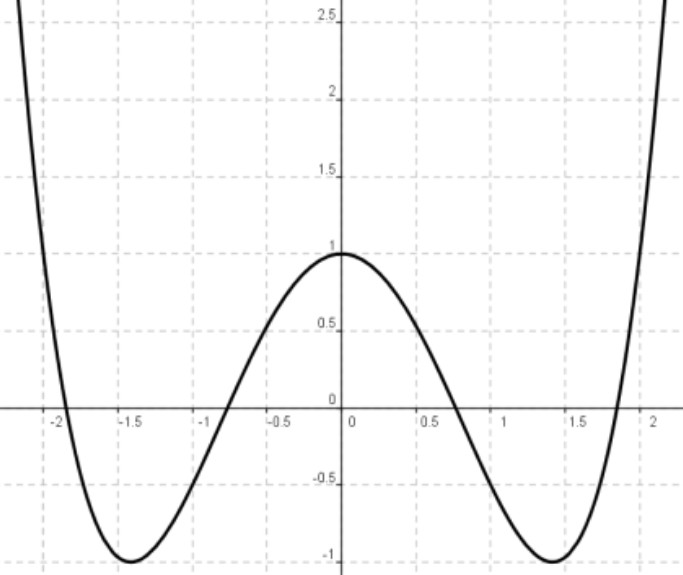
\includegraphics[width=0.7 \linewidth]{Q11_210111_4.jpg}
%  \end{center}
%\end{figure}




\begin{figure}[H]
  \centering

    \subfloat[A]{
          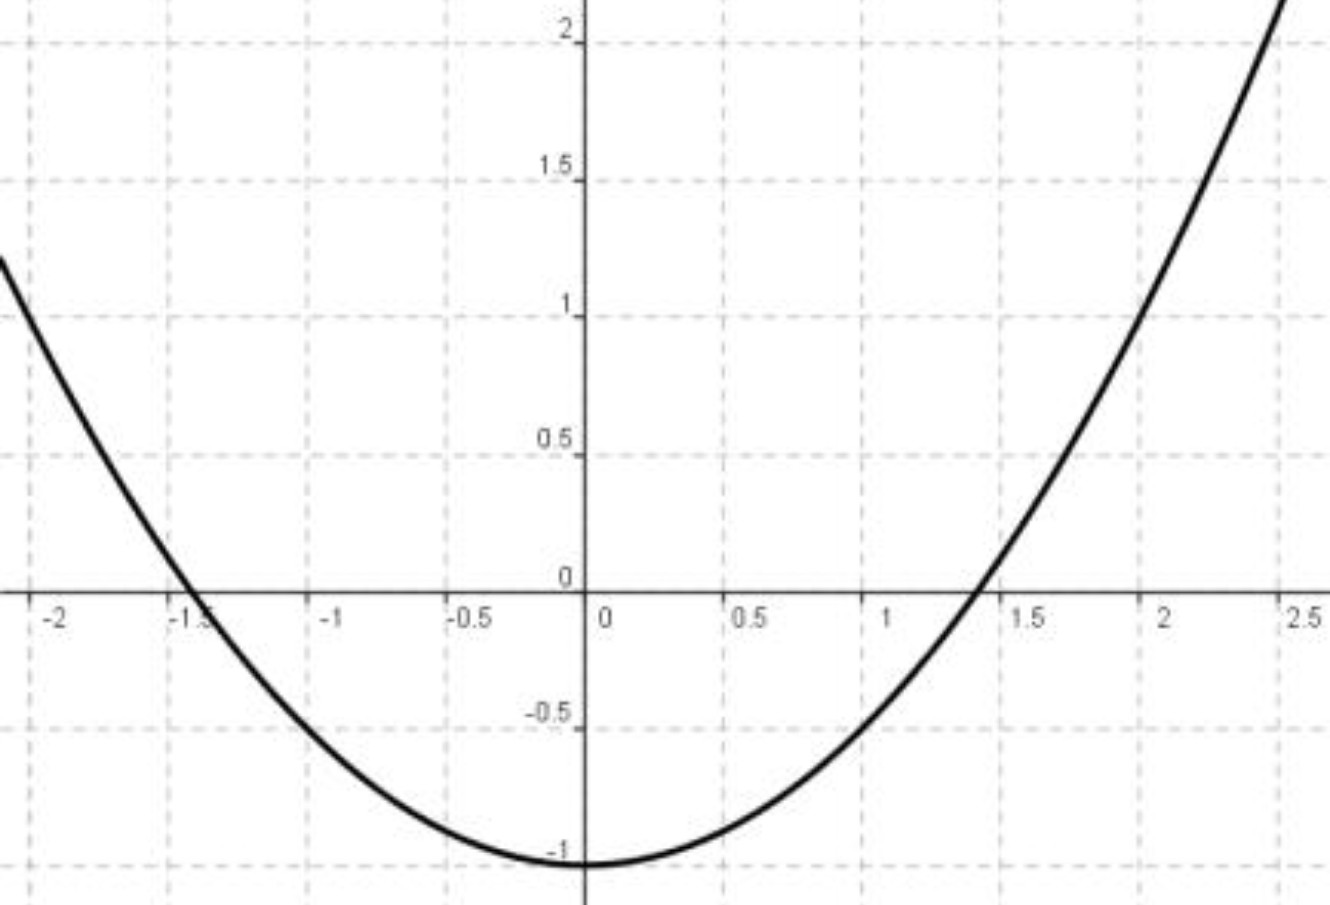
\includegraphics[width=0.3 \linewidth]{Q11_210111_4A.jpg}
        }
    \subfloat[B]{
          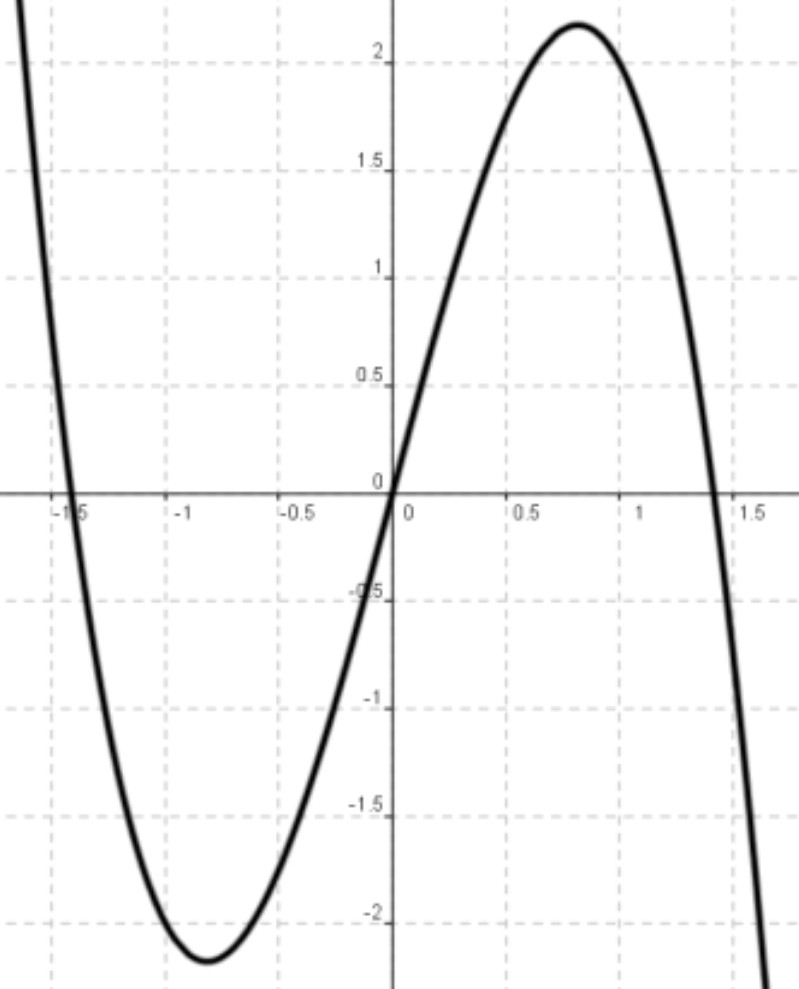
\includegraphics[width=0.3 \linewidth]{Q11_210111_4B.jpg}
    }      %<------------
\end{figure}


\begin{figure}[H]
  \centering

    \subfloat[C]{
          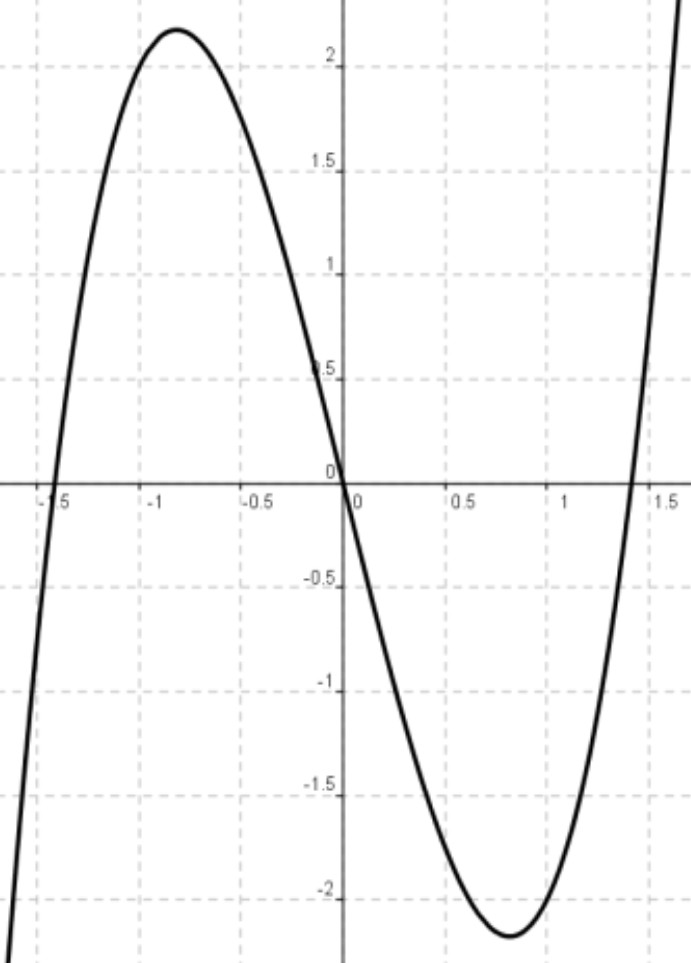
\includegraphics[width=0.3 \linewidth]{Q11_210111_4C.jpg}
    }      
    \subfloat[D]{
          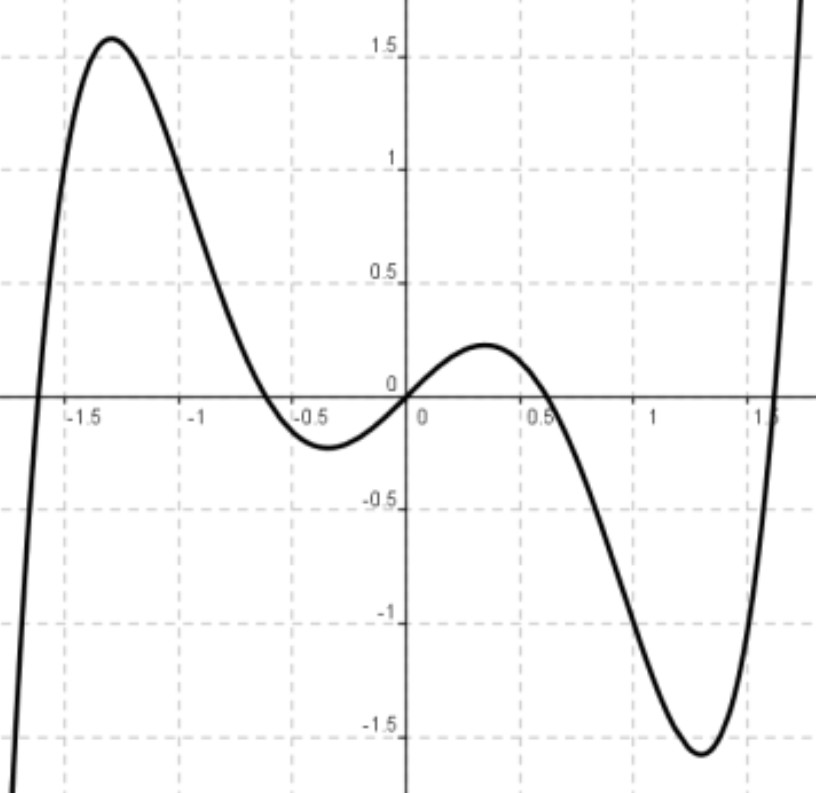
\includegraphics[width=0.3 \linewidth]{Q11_210111_4D.jpg}
    }      
    \subfloat[E]{
          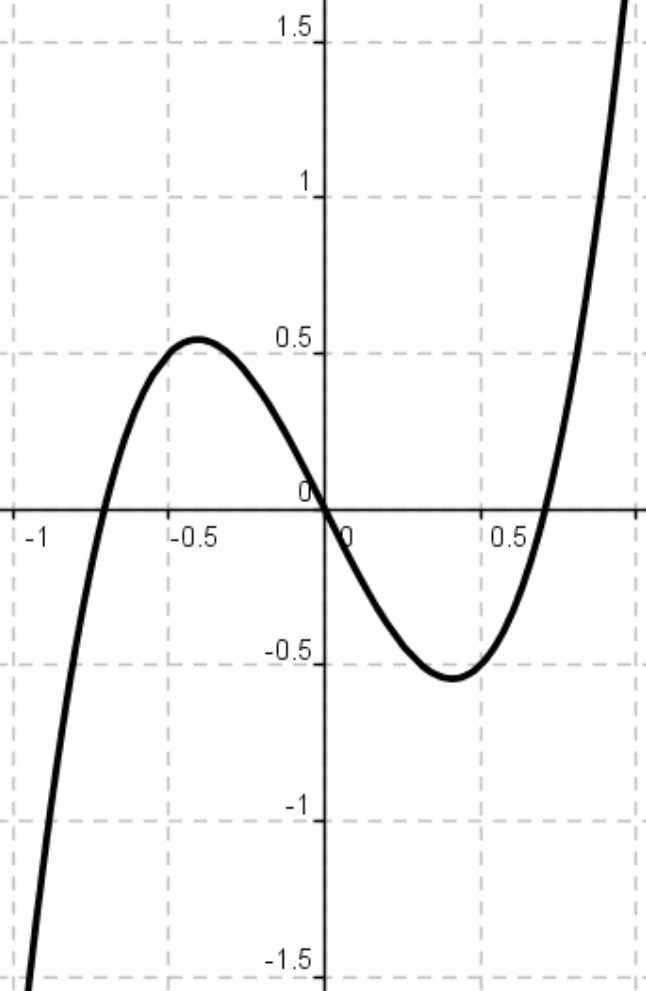
\includegraphics[width=0.3 \linewidth]{Q11_210111_4E.jpg}
    }      
\end{figure}

\begin{flushright}6 BE \end{flushright}
\newpage





\Aufgabe {5:} 

Bestimmen Sie jeweils einen Funktionsterm $u(x)$ so, dass $f(x)=u(v(x))$ ist und berechnen Sie die Ableitung von $f(x)$. Erklären Sie im Allgemeinen, wann sind die Funktionen umkehrbar und berechnen Sie die $x$-Werte, für welche die Funktionen $f(x)$  jeweils umkehrbar sind. 


\begin{enumerate}[label={\alph*)}]
  \item $f(x)=(5x-10)^2; \quad v(x)=x-2$
  \item $f(x)=cos\sqrt{2x-1}; \quad v(x)=2x-1  \quad  $ für $x \geq 0,5$ 
\end{enumerate}

\begin{flushright} 9 BE \end{flushright}
\vspace{0,8cm}


\centerline{Viel Erfolg}
%\enlargethispage{2\baselineskip}

%\addtolength{\voffset}{-2cm}




%\begin{tikzpicture}
%\draw [very thin, black, step=0.5cm] (0,0) grid +(15,18);
%\end{tikzpicture}




%%%%%%%%%%%%%%%%%%%%%%%%%%%%%%%%%%%%%%%%%%%%%%%%%%%%%%
%%%%%%%%%%%%%%%%%%%%%%%%%%%%%%%%%%%%%%%%%%%%%%%%%%%%%%
\end{document}
